\chapter{Structure Art and Pure Mathematics (1960)}

In some art---music, visual art, poetry, and the rest---there is a tendency for 
"structure" to predominate. When structure tends to predominate in art, then \emph{if} the 
artist wants the interest of the structure to predominate, wants to communicate the 
interest of the structure, I will say that the art is "structure art." Much structure 
art is a vestige of Serious Art; for exemple, of medieval music, which was conceived 
to be a metaphysical science. Now consider, for example, a piece of structure music, 
a serial piece. The "structure" of the piece is \emph{not} (in) the sounds in (a performance 
of) the piece. It is a categorization of the sounds, that represented by the score 
together with that typically given in the first instance by the composer in an "analysis" 
of the "piece" (actually the analysis is more a part of the piece). Thus if I speak 
of the "intended structure" of a piece it will be the composer's categorization; and I 
will speak of others' categorizations, the audiences' categorizations, as "associated 
structures" of the piece. (To some extent the composer can work to the audience's 
background so that one association is more probable than another.) Many structure 
artists do claim "that the structure (particulerly the intended structure) is in the 
sounds" in that, for example, there is an objective relation between the categorization 
and the sounds. This claim is unjustifiable; I will return to it later. There is an 
important division of structure art into two kinds, exemplified by the fugue and total 
serial music, according to how the structure is "appreciated." In the case of a fugue, 
one is aware of its structure in listening to it; one mentally imposes "reletionships," 
a categorization (hopefully the intended one) on the sounds while listening to them 
that is, there is an "associated artistic structuring by oneself." In the case of total 
serial music, the structure is such that this cannot be done; one just has to read an 
"analysis" of the music, a specification of relationships. Incidentally, there is 
another, less important kind of art in which the important thing is categorization; 
the art involving conceptual cleverness, play with the concepts of the art-form such as, 
in music, "the score," "performer versus listener," "playing a composition." In 
structure poetry, there is a lack of concern with syntacticel structure. The poetry 
is mere phonemes or graphemes with an artistic structure. 

The following is an attempt at a formal definition of "artistic structure." 
The artistic structure of a production is a division or segmentation of the raw work 
(the body of material), a grouping of the segments, and a "weighting" of the subgroupings 
in this grouping (according to their"structural importance"); that is, it is a system 
of definitions. When structure is regarded as the most important aspect of the 
production, the production is merely a diagram illustrating the description of its 
structure. Certain pieces of music are merely acoustical diagrams of their structures. 
Such a production consists of the production proper together with a concept poem, a 
body of definitions. Here is a canonical method of specifying such structures. 
Given the raw work, the informal description of its structure is as follows. The 
segments are blocks of color; the first two are grouped together, and each of the 
others is grouped separately; the weights of the successive groups are $5, 2, 4, 2, 4$
(2 is the weight of \eg\ a bridge passage in music). The formal specification is 
$(AB)_5(C)_2(D)_4(E)_2(F)_4$;  that is, the production is structurally a "$(AB)_5(C)_2(D)_4(E)_2(F)_4$."


The method, then, is that the terminology for a certain structure is formed from 
letters corresponding to segments, parentheses to indicate grouping, and numerical 
subscripts to indicate weights. (Does the method need to be elaborated to take into 
account relations between segments?) It can be seen that this kind of structure is 
definitional, stipulational, like logical syntax; it is not intuitive and statistical 
like an individual's use of inflection in speech. I now turn to the analyses of 
the structure of a production made by critics, what I call "associated definitions of the 
structure" (in line with the terminology of the previous paragraph), Consider the 
following examples. 

{ \centering
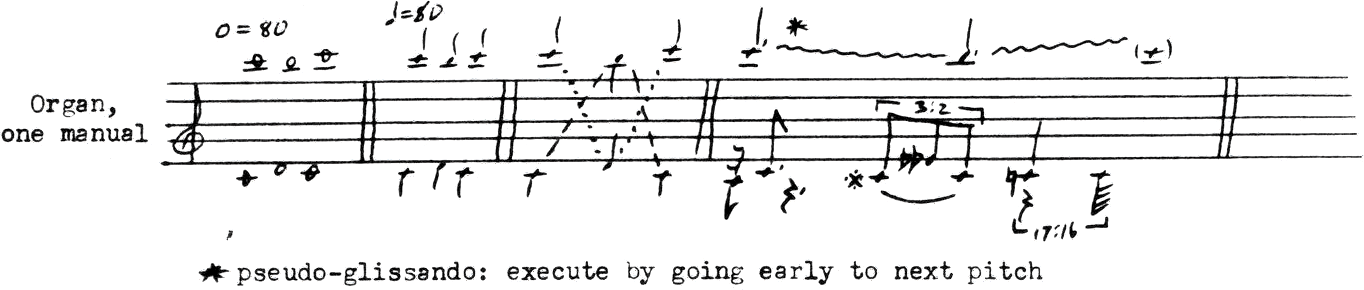
\includegraphics[width=4in]{img/structure_art}\par
}

In each example, the actual sounds, the body of material, is exactly the same. 
The difference is in the different structures defined on the material. The examples 
substantiate my contentions thet the structure is not in the sounds; that the composer's 
analysis of the piece is really a definition and a part of the piece; and that the 
critics' analyses of the structure are definitions attached to the piece, not discoveries 
of intrinsic properties of the sounds. As another example, consider the difference 
between hearing the "Sanctus," \opustitle{Missa Prolationum} of Ockhegem, in no meter (by 
a non-European listener), in one meter (by a lay European listener), and in four 
meters (the intended structure). Arguments such as the one over whether the structure 
of Webern's music is "really" motivic or serial are absurd, since Webern himself did not 
define this point. Many academic structural analyses of art have been irrelevant 
to the aesthetics of the works. 

The purpose throughout all this art is dual; structure or concept art tries to be, 
first, music, visual art, or whatever (which suggests that it is to be listened to, or 
looked at), \emph{and}, something else entirely, to be valuable for its structure or conceptual 
cleverness. Then when the structure is "hidden," "unexperiencable," when it can only be 
appreciated by reading the "analysis," why put emphasis on the body of sound, light, or 
whatever, why listen to structure music, why look at structural visual art, why even call 
them "music," "visual art"? Why not throw away the bodies of sound, light, or whatever, 
and keep the "analyses" of the structure as the works of art? In general, logic, and 
experience (with the results of the artists' efforts), show that the dual purpose of 
structure art consists of irreconcilable objectives; that one can be attained only at the 
other's expense. Which objective are the structure artists trying to attain?---they 
obviously have no idea. Structure art represents obsolete, confused categories of 
activities, categories which by now are obscurantist. Structure (or concept) music, 
for example, needs straightening out, first, by ceasing to call it "music," and starting 
to say thet the sound (or activity) is used only to carry the structure or conceptual 
cleverness, and that the real point is the structure or conceptual cleverness---the 
categorization---and then it will be seen how limited, impoverished the structure of 
these productions trying to be music are. When you make the change, then you are led 
to a far more consistent, integral activity, the same one arrived at below through 
a consideration of pure mathematics. Games of intellectual skill such as chess fall 
into this same category; since, after all, they can be regerded as formalist mathematics. 

Neryt I will discuss pure mathematics. Originally, mathematics was a system of 
beliefs, a doctrine, about the entities numbers, points, polygons, and so forth (Pythagoras, 
Euclid, Platonic geometry). As mathematicians became skeptical, and thus less desirous 
of resting the importance of mathematics on the validity of these beliefs, they changed 
their minds about what the purpose of mathematics is. The purpose became for the theorems 
to be true if the axioms are. In the nineteenth century, as a result of e.g. the ideas 
of Riemann, they became unconcerned to claim that their axioms are true. They began 
to say that the value of mathematics is "aesthetic." Here is when mathematics becomes 
a subject for this essay; when it becomes pure mathematics, when its value is not claimed 
to be that of technology or natural science, but rather more an aesthetic value, when it 
becomes "adoctrinal culture." Mathematics becomes something to be considered alongside art. 
When I became interested in contributing to pure mathematics, for reasons of taste I wanted 
to de-emphasize discovery in mathematics, mathematics as discovering theorems and proofs. 
(Such discovery bored me.) The first way I thought of to de-emphasize discovery was that 
since the value of pure mathematics is now regarded as conceptual interest, aesthetic 
rather than scientific value, why not try to make up aesthetic theorems, without considering 
whether they are true. The second way was to find that the conventional claim that 
theorems and proofs are discovered is unjustifiable; I will return to this point later. 
In the twentieth century, as a result of the ideas of Hilbert, and then Carnap, 
mathematicians became unconcerned to claim that mathematical "statements," the 
mathematical object language, are (substantive) assertions having truth value (as are 
English statements). Rather, they are "merely" series of signs formed according to 
certain rules: formalist mathematics. Then my third way of de-emphasizing discovery was 
to open up unexplored regions of formalist mathematics. The resulting mathematics still 
had statements, theorems, proofs, but the latter weren't "discovered" the way they 
traditionally were. 

Now exploration of the wider possibilities of pure mathematics opened up by me 
tends to lead beyond the form of "making statements," "proving," and the like, so thet 
the term "pure mathematics" becomes completely incongruous. The category of pure 
mathematics---a vestige ultimately of the old system of beliefs canonized by Plato 
(hence the form of statements, proving, and the like)---is an obsolete category. My 
contributions to pure mathematics lead to an integral, general activity of which the 
point is categorizations (having the value of being "well-formed"); the contributions 
need to be classified as such an activity rather than as pure mathematics to escape 
confusion, Traditional mathematics (mathematics as discovery), reformulated, explicated 
to take my findings into account, would be an untypical, small but intensively developed 
part of such an activity. 

The proponents of structure art, pure mathematics, and chess make similar claims 
for them. I have mentioned the claims that structure is an objective property of things; 
and that mathematical theorems and proofs are discovered; and there is a similar claim for 
games of intellectual skill. Two important notions associated with these fundamentally 
identical claims require comment. There is the notion that contribution to structure 
art, pure mathematics, and chess requires high intelligence, the discovery of implications; 
the notion of intelligence as the ability to discover implications. Then, there is the 
notion that structure (as in mathematics pre-eminently) is an objective property of things, 
capable of discovery, demonstration, rational cognition---with particular reference 
to language, art, and the like---whereas meaning, expression, and emotion are not. 
(These pretensions are traditionally an essential aspect of structure art, pure mathematics, 
and chess.) Both notions come down to the belief that there can be an objective relation 
between a name and its referents; for example, an objective relation between the 
metamathematical term "true theorem" and certain theorems, or an objective relation 
between "having serial structure" and a body of sound, or between "checkmate" and 
checkmates. As I said, these notions are discreditable, as can be seen from my 
\essaytitle{Philosophy Proper} and \essaytitle{Primary Paradox}. Thus the notion of intelligence, pretension 
of intellectual superiority, as what mathematicians, chess players, and the like have; 
and the prejudice in favor of structure; cannot be defended. It is about time that 
these notions be discarded. 


